\documentclass[../main.tex]{subfiles}
\graphicspath{{\subfix{../images/}}}

\begin{document}
	\chapter{Scelte organizzative}

	\section{Introduzione}
	Ora analizzeremo alcune scelte che stanno alla base del organizzazione dei sistemi informativi nelle aziende.
	\begin{itemize}
		\item Le forme di reperimento/costruzione del sistema informativo.
		\item I tipi di figure informatiche.
		\item Le scelte strategiche sull'infrastruttura.
		\item Le problematiche legate all'unteroperabilità del servizio fornito dal sistema.
	\end{itemize}

	\section{Costruzione del sistema informativo}
	Al giorno d'oggi esistono tre modalità:
	\begin{enumerate}
		\item \textbf{Make: } costruire interamente il proprio sistema informativo.
		\item \textbf{Buy: } comprarlo dall'esterno.
		\item \textbf{Outsource: } darlo in gestione ad un'ente esterna.
	\end{enumerate}
	Nel mondo reale però non si adotta una sola tecnica ma solitamente si punta a mescolarle.

	\subsection{Make}
	Questa scelta molto in voga alla nascita dei primi sistemi informativi è oggi usata solo da grandi aziende.\\
	Con questa opzione l'azienda sviluppa tutto il software necessario e i servizi, l'unica cosa comprata dall'esterno per ovvi motivi è l'hardware.
	\begin{itemize}
		\item Costi fissi molto alti: l'azienda deve possedere uno staff preposto allo sviluppo e alla gestione di tale software.
		\item Investimenti consistenti: oltre all'acquisto di tutta l'infrastruttura per poter lavorare l'azienda deve anche comprare hardware ed eventuale software.
		\item Struttura che non si confronta col mercato: uno degli aspetti più critici, essendo il software in una specie di "monopolio" per l'azienda che lo ha prodotto non è soggetto a nessun miglioramento dato dalla competizione del mercato.
		\item Le soluzioni tendono a diventare obsolete: questa problematica è fortemente legata alla precedente.
		\item Tempi di soluzione veloci per problemi banali ma molto dilatati per problemi complessi.
		\item Mantenimento interno del "know-how": ovvero solo l'azienda sa come funziona il software che ha prodotto quindi in casi di riservatezza molto alta questo risulta essere un punto a favore non da poco.
		\item I modelli organizzativi sono mappati in modo molto puntuale perchè il software è sviluppato ad-hoc, questo però non è sempre un vantaggio in quanto molte volte le soluzioni più generali risultano essere molto più efficenti.
	\end{itemize}

	\subsection{Buy}
	Questa scelta prevede l'acquisto del proprio SI da un'azienda specializzata ed esterna, solitamente questa scelta era adottata da molte PMI ma con l'introduzione degli ERP anche dalle grandi aziende.
	\begin{itemize}
		\item E' comunque presente, seppur in dimensioni ridotte, una struttura interna all'azienda per poter dialogare e sincronizzare i fornitori.
		\item Parziale smobilizzazione degli investimenti iniziali dell'azienda infatti non viene pagato lo sviluppo del software.
		\item Concetrazione sul core business: non dovendo pensare allo sviluppo del SI.
		\item Dipendenza da una struttura esterna, solitamente i tempi necessari per cambiare fornitore sono molto lunghi e le software house detengono molto potere contrattule.
		\item Maggior flessibilità rispetto al "make", un fonrnitore essendo sul mercato deve avere una dimensione adeguata per poter seguire i propri clienti.
		\item Fuoriuscita di parte del "know-how" aziendale: per necessità la software house dev conoscere i processi e i dati interni di un'azienda.
		\item Mancanza di proprietà del software: tutte le spese connesse ad un software non portano alla proprietà di esso, solamente alla detenzione di una licenza di uso.
		\item Possibilità di interventi limitata: ovviamente se insorgono problemi deve essere il fornitore ad occuparsene e non l'azienda direttamente.
		\item Continua aderenza al mercato essendo il fonitore immerso nel mercato.
		\item Modelli organizzativi mediati: solitamente la software house ha la propria soluzione che deve essere personalizzata per l'azienda.
		\item Difficoltà nell'interazione con più fornitori: spesso dialogare con molti fornitori per poter opeare sul sistema informativo da loro comprato è dispendioso di risorse.
	\end{itemize}
	\begin{center}
		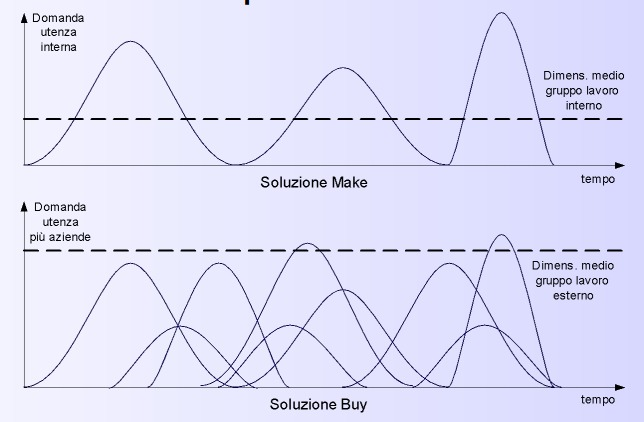
\includegraphics[scale=0.5]{opzione_buy.png}
	\end{center}
	
	\subsection{Outsource}
	Questa scelta organizzativa consiste nel portare all'esterno tutto quello ch riguarda lo sviluppo/gestione/mantenimento del sistema informativo, pagando un canone mensile opper con tempi più lunghi.\\
	Si noti che l'outsourcing è concettualmente diverso dal hosting in cui si porta all'esterno l'infrastryttura ma si mantiene il controllo del softwre che solitamnete è gestito con la "buy" e dal body-rental in cui si affitta il personale di un'altra azienda nei periodi i maggior richiesta.
	L'opzione "outsource" inizialmente circoscritta alle grandi aziende è ad oggi usata da molte PMI, possiamo trovare sistemi in outsourcing completo nelle grandi aziende oppure soluzioni parziali nelle PMI.\\
	La crescentre complessità dei sistemi ed il bisogno di garantire sicurezza e continuità rendono pocco conveniente creare un servizio all'interno di un'azienda.
	\begin{itemize}
		\item Costi variabili: non essendoci personale dedicatio i costi risultano fissi, a meno di cambio del canone di utilizzo.
		\item Smobilizzazione totale degli investimenti: non essendoci alcun investimento in infrastruttura, hardware e software.
		\item Voncolo completo con il fornitore del servizio, se il fornitore chiudesse l'azienda sarebbe privata del proprio SI.
		\item Maggior flessibilità rispetto al "make" perchè è spesso presente una possibilità di scalare i servizi ricevuti.
		\item Esposizione di tutto il know-how perchè completamente affidato a terzi.
		\item Perdita di controllo sulla potenza contrattuale che un fornitore può esercitare sull'azienda.
		\item Possibilità di intervento diretto assente.
		\item Esattamente come nel modello "buy" si è molto più aderenti al mercato e con modelli organizzativi mediati.
	\end{itemize}

	\section{Posizionamento del sistema informativo}
	\subsection{Figure professionali}
	Le figure professionali "informatiche" che operano all'interno di un'azienda sono legate alla "maturità informatica" che un azienda possied,
	possiamo considerarne quattrio livelli.

	\subsubsection{Livello 1}
	Il team è composto da un ristretto numero di persone con compiti molto diversificati e spesso si occupano anche di altro, questi team presentano una struttura che è prettamente orizzontale senza la presenza di una figura dirigenziale.\\
	Spesso questo livello è presente solo nella prima fase di automazione di un'azienda, nella quale si ha una visione a breve termine con poco o nessun budget.

	\subsubsection{Livello 2}
	In questo livello iniziano a delinearsi dei ruoli ben precisi, con anche dei ruoli di responsabilità come l' EDP manager (Electronic Data Processing).\\
	I ruoli delineati seguono tre filoni principali con responsabilità diverse:
	\begin{itemize}
		\item Il sistemista, che gestisce e mantiene l'infrastruttura tecnologica.
		\item L'analista, supporta gli utenti esaminando le nuove esigenze che emergono dall'evoluzione dell'azienda.
		\item Il programmatore che si occupa dello sviluppo di nuove applicazioni, questa figura è sempre presente nell'opzione "make" ma totalmente nelle opzioni "buy" e "outsource".
	\end{itemize}
	Spesso le funzioni di analista e programmatore sono accorpate sotto il nome ingegnere del software.
	\begin{center}
		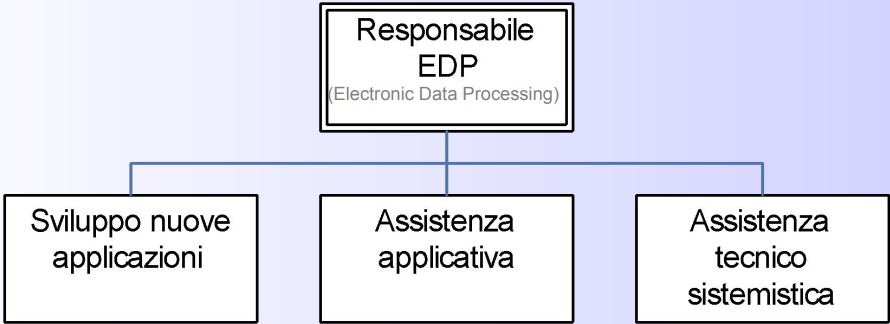
\includegraphics[scale=0.3]{figure_professionali_livello_2.png}
	\end{center}

	\subsubsection{Livello 3}
	La struttura inizia a diventare più complessa con la creazione di una nuova ala che si occupa delle nuove tecnologie, viene costituita una vera e propria direzione e quindi viene assunto un ruolo strategico nei piani dell'azienda.
	\begin{center}
		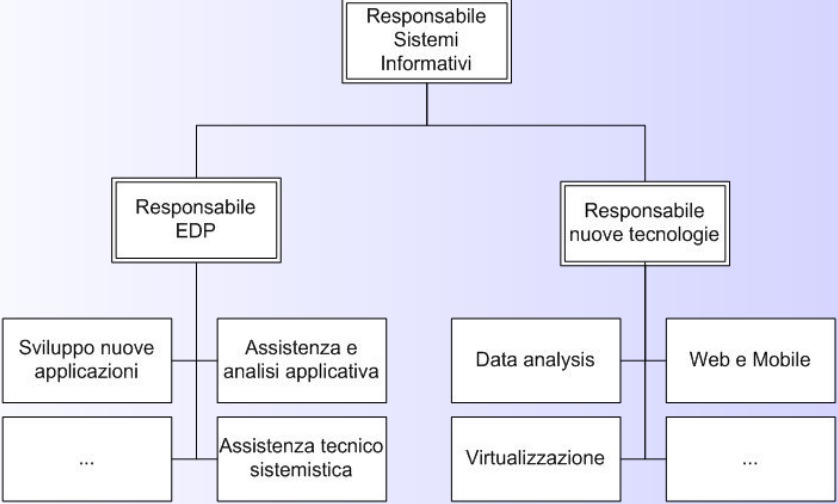
\includegraphics[scale=0.3]{figure_professionali_livello_3.png}
	\end{center}

	\subsubsection{Livello 4}
	E' il livello più articolato nel quale tra il responsabile e i vari dirigenti si vanno a delineare diverse figure come:
	\begin{itemize}
		\item Segreteria.
		\item Pianificazione.
		\item Privacy e sicurezza.
		\item Documentazione e standard.
		\item Definizione e controllo del budget.
	\end{itemize}
	Dipendentemente da caso a caso possono nascere ulteriori ruoli.

	\subsection{Posizionamento nell'organigramma}
	E' importante che oltre alla creazione di figure professionali apposite il settore ICT venga posizionato in modo corretto all'interno di un'azienda.\\
	Si identificano quindi tre macro categorie anche se spesso si utilizano soluzioni miste.
	
	\subsubsection{Servizio all'amministrazione}
	Questa visione vede i SI solo sotto una luce amministrativa e di misurazione mettendo in secondo piano la getsione e organizzazione del core business.\\
	Il SI vien così usato solo come archivio di eventi aziendali successi.

	\subsubsection{Servizio alle altre aree aziendali}
	Il settore di gestione del SI viene visto come pari di tutte le altre direzioni aziendali permettendo quindi di poter essere di supporto a queste ultime.

	\subsubsection{Servizio all'Organizzazione}
	Gerarchia usata dalle grandi aziende in cui è molto importante formalizzare i processi.\\
	Viene identificata un'area apposita che organizza complessivamente l'azienda, e si assegna ad essa la gestione del SI, questa nuova direzione proteggetterà e implementerà i modelli organizzativi aziendali.

	\section{Infrastrutture: dai sistemi centralizzati ai cloud}
	Gli "antichi" sistemi formati da un' unità centrale con più terminali collegati, ha lasciato il posto ad architettura client-server le quali hanno lasciato a loro volta il posto a tecnologie più complesse grazie a Internet.\\
	La virtualizzazione ha portato ad eseguire su un'unica macchina fisica più software in parallelo, i dispositivi mobili hanno portato ad un aumento esponenziale degli host collegati, l' IoT ha portato ad un aumento degli elenti generatori di informazioni e la rete wireless ha reso qualsiasi punto geografico un potenziale punto di accesso.\\
	Questa crescita ha portato con se:
	\begin{itemize}
		\item Una crescita nelle diffficoltà legate alla getsione dell'infrastruttura.
		\item Il bisogno di garantire l'integrità e disponibilità del sistema.
	\end{itemize}

	\subsection{Dal server locale ai server cloud}
	Da alcuni anni si sta migrando verso un'infrastruttura in cloud, anche grazie all'efficenza ed alla stabilità delle connessioni.\\
	I sistemi in cloud presentano molti vantaggi come:
	\begin{itemize}
		\item Non è necessario investire grandi somme nell'acquisto di software e hardare.
		\item La maggior parte della gestione dell'infrastruttura è demandata al fornitore del servizio.
		\item Il sistema informativo risulta accessibile 24/7 e da qualsiasi parte del globo.
		\item Le aziende possono accedere a molti servizi ch con l'opzione "make" avrebbero costi proibitivi.
	\end{itemize}
	Purtroppo le soluzioni cloud vincolano il funzionamento del SI alla presenza di una connessione ad internet.

	\section{Interrompibilità del servizio informatico}
	Troppo spesso nelle aziende non del settore i dirigenti non considerano i rischi che derivano da un'eventuale interruzione del servizio del SI, le interruzioni possono portare in tempi molto brevi ad una paralisi totale delle attività gestite dal SI.\\
	La "continuità operativa" cioè il quasi azzeramento del rischio di interruzione è un bislogno che ogni azienda dovrebbe avere.

	\subsection{Problemi dipendenti dall'hardware}
	L'hardware essendo un apparato fisico è soggetto come ogni altra cosa a guasti, soprattutto nelle sue parti mobili.\\
	In caso di gravi guasti il tempo di ripristino del servizio è molto importante, perchè oltre a rispristinare il pezzo guasto si devono recuperare i dati.\\
	Una componente che molto spesso si rompe è l'unità di memoria secondaria (hard-disk), possiamo quindi usare più dischi per sfruttare i RAID (Redundant Array of Indipendent Disks).\\
	Un'altra opzione, molto più difficile da implementare, è l'hot-swap dei dischi in cui si può sostituire un disco mantenendo la macchina in funzione.\\
	Le tecnic he prima descritte comprono però solo parti duplicate del sistema infatti se per caso viene meno la RAM il sistema vado down in ogni caso, per le applicazioni "mission critical" dove non ci può fermare è importante implementare architetture così dette "fault tollerance" che hanno un livello di ridondanza molto elevata.\\
	Come accennato prima oltre a ripristinare la parte danneggiata dobbiamo ripristinare i dati temporaneamente persi, entrano in gioco varie tecniche di "back-up", nelle quali si creano copie delle informazioni che verranno immagazinate e storicizzate, in alcuni casi estremi è perfino possibile fare compie dell'intero sistema per velocizzare la "disaster recovery".

	\subsection{Problemi dipendenti dal software}
	
\end{document}